\documentclass{article}

\usepackage{amsmath}
\usepackage{amsthm}
\usepackage{eucal}
\usepackage{amssymb}
\usepackage{color}
\usepackage{tikz}
\usetikzlibrary{shapes,arrows.meta,backgrounds}
\usepackage{etoolbox}
\usepackage{url} % for urls in bibliography
\usepackage[parfill]{parskip} % no paragraph indents, leave blank line
\usepackage{graphicx}
\usepackage{subcaption}
\usepackage{listings}
\usepackage{xifthen}% provides \isempty test

\graphicspath{ {./drawio/} }

% Need this to keep the space before theorems when using parfill parskip
% https://tex.stackexchange.com/questions/25346/wrong-spacing-before-theorem-environment-amsthm
\begingroup
    \makeatletter
    \@for\theoremstyle:=definition,remark,plain\do{%
        \expandafter\g@addto@macro\csname th@\theoremstyle\endcsname{%
            \addtolength\thm@preskip\parskip
            }%
        }
\endgroup

\DeclareRobustCommand{\rchi}{{\mathpalette\irchi\relax}}
\newcommand{\irchi}[2]{\raisebox{\depth}{$#1\chi$}} % inner command, used by \rchi

\usepackage{mathtools}
\usepackage{bm}
\usepackage{stmaryrd} % for llbracket and rrbracket

\theoremstyle{definition}
\newtheorem{example}{Example}[section]
\newtheorem{defn}{Definition}[section]

\newcommand{\adj}[1]{\llbracket #1 \rrbracket} 
\newcommand{\enf}[1]{[#1]} 

\newcommand{\holds}[3]{#1 %
  \ifthenelse{\isempty{#2}}{}{: #2} %
  \ifthenelse{\isempty{#3}}{}{\mapsto #3} %
} 
\newcommand{\alloc}[1]{( #1 )} 
\newcommand{\guar}[2]{( #1 | #2 )} 

\newcommand{\finalizable}[3]{[#1 \mapsto #2]_{#3}}
\newcommand{\transfer}[3]{\mathcal{T}(#1, #2, #3)}
\newcommand{\claim}[3]{\mathcal{C}(#1, #2, #3)}


\title{Nitro Protocol}
\author{Tom Close}

\begin{document}

\maketitle
\begin{abstract}
  State channels are an important technique for scaling blockchains, allowing a fixed set of participants to trustlessly execute a series of state transitions off-chain, to determine how a set of assets should be distributed between them.
  In this paper we present constructions that allow state channels to be fund one another, reducing the number of on-chain deposits required from one per channel to one per participant.
  Unlike in previous constructions, channels funded by other channels operate identically to channels funded on-chain, making it easier to reason about the applications that run within them.
  We develop the logic to prove the correctness of our constructions.
\end{abstract}

\section{Motivation}

State channels are an important technique for scaling blockchains.
In a state channel, a fixed set of participants execute a series of state transitions off-chain, to determine how a set of assets should be distributed between them.
By allowing participants to execute multiple transitions off-chain, the state channel removes load from the blockchain, allowing the blockchain to support the same level of activity with fewer transactions.

State channels are relatively unique amongst scaling techniques in that they provide a way to run arbitrary state update protocols, instead of just providing a method for realizing transfers off-chain.
- TODO?

Beyond scaling, state channels bring instant finality to blockchain transactions:
in many situations, value can considered to be transferred at the moment when a state channel update is received.
The receiver does not need to wait for the transaction to be mined, safe in the knowledge
that they have the right to claim the assets on-chain at a future point of time of their choosing.

In their naive form, each state channel needs to have a corresponding \textit{state deposit} - a set of assets held in escrow on-chain, to be distributed according to the outcome of the channel.
Each time a state channel is opened at least one participant needs to perform an on-chain transaction to transfer assets into the state channel, and each time it is closed at least one participant must perform an on-chain transaction to claim their share.
This limits the effectiveness of state channels as a scaling solution, making it only suitable for relatively uncommon case where a large number of transactions are done between a single group of participants.
We refer to these naive channels as \textbf{direct channels}, as they are supported directly by funds held on the blockchain.

\subsection{Ledger Channels and Virtual Channels}


Ledger channels allow multiple channels between a given set of participants to be supported by a single on-chain deposit.
Importantly, these channels still update independently to one another, even though they are funded by the same deposit.

As an example of what ledger channels enable, suppose Alice and Bob want to play a game of chess and that
they already have an existing ledger channel open between them.
The winner of the game of chess should receive 2 coins from the loser and $\rchi_L$ currently holds
5 of Alice's coins and 5 of Bob's.

\begin{center}
  \includegraphics[scale=0.5]{turbo_start} % TODO: tikz
\end{center}

Alice and Bob proceed by creating a new channel for the chess game with the appropriate starting state.
They then update the ledger channel to allocate funds to these games.

\begin{center}
  \includegraphics[scale=0.5]{turbo_open} %TODO: tikz
\end{center}

Once the funds are allocated, they are free to play the game of chess.
Updates to the chess channel are independent from updates to and to
any other sub-channels that are potentially funded by it. 
Alice wins the chess game, so the final state in the chess channel allocates all the
funds to her.

\begin{center}
  \includegraphics[scale=0.5]{turbo_close} %TODO: tikz
\end{center}

To close the chess channel off-chain, Alice and Bob update the state of the ledger channel to absorb the outcome of the game.

\begin{center}
  \includegraphics[scale=0.5]{turbo_finish} %TODO: tikz
\end{center}

Virtual channels go one step further than ledger channels, allowing a state channel to be opened between two participants who do not share an on-chain deposit, but instead have a connection in common, with whom they both have a channel open with.

As an example, suppose that Alice wants to open an $\{A:5, B:5\}$ chess game with Bob, but they do not share an existing ledger channel.
Alice does, however, have an $\{A:5, C:5\}$ ledger channel open with Carol and Bob and Carol have a $\{B:5, C:5\}$ ledger channel open too.

By using a virtual channel, Alice and Bob to open their chess game, using their existing ledger channels with Carol, without the need for any on-chain transactions.
Suppose that Alice wins all of the funds in the channel, so that the final outcome is $\{A: 10, B: 0\}$.
Alice and Bob can also close their chess game off-chain, rebalancing through Carol, so that the final state of the ledger channels is $\{A: 10, C: 0\}$ and $\{B: 0, C: 10\}$.

In this interaction, Carol contributed 10 of her coins at the beginning, which had to remain locked while Alice and Bob were playing.
She got those 10 coins back but they were distributed differently between the her ledger channels.
By locking up her coins for a period of time, she enabled Alice and Bob to play chess entirely off-chain.

One good way of summarising the differences between these three different approaches is to look at the number of on-chain deposits required in each of them:
\begin{itemize}
  \item \textbf{Direct channels}: on the order of one on-chain deposit per channel
  \item \textbf{Ledger channels}: on the order of one on-chain deposit per group of participants
  \item \textbf{Virtual channels}: on the order of one on-chain deposit per participant
\end{itemize}
Virtual channels hold the biggest potential in terms of scaling, requiring only one on-chain deposit per participant.

\section{Existing work}

TODO
\subsection{Our contribution}

- virtual and ledger channels
- channels are unrestricted
- no time limits or special update rules due to being in a virtual channel

\section{State Channel Background}

In this section, we introduce the state channel concepts necessary to understand the rest of the paper.

\subsection{Operating vs. Funding State Channels}

At the heart of our approach lies the decision to make the funding of a state channel independent from its operation.

We view a state channel as a device for allowing a fixed set of participants to determine how a set of shared assets should be split between them.
We refer to the set of instructions that determine how the funds should be split as the  \textbf{outcome} the state channel.
We define the \textbf{operation} of a state channel to be the process by which the channel reaches an outcome. 
The \textbf{funding} of a state channel is the method of ensuring that the outcome is honoured on-chain.

Specifying the operation of a state channel involves specifying the format of the states and the update rules that define the allowed transitions between these states.
Specifying the operation also involves defining the rules surrounding on-chain challenges and the ways to respond to them.
The ForceMove protocol is an example of a protocol that specifies the operation of a state channel.
In this paper, we will not specify the operation of state channels, instead leaning on ForceMove where required.

Specifying how state channels are funded involves specifying how funds are held in escrow on the chain, how they can be deposited and how they can be claimed according to the outcome of a state channel.
As we will see in this paper, it can also involve specifying the rules for how the outcomes of multiple channels interact, which enables channels to be funded and defunded without on-chain operations.
In the ForceMove paper, all funding was done by the \textit{SimpleAdjudicator}, which only allowed for direct channels between participants.

Decoupling the funding of the channel from its operation has several advantages.
Provided that a channel is funded, its operation is completely independent from the other channels in the system.
The source of funding for a channel can even change from off-chain to on-chain, all without interrupting the operation of that channel.
Overall, by forcing channels to operate independently and only be coupled through funding relationships, it becomes a lot easier to reason about the behaviour of any applications running within a state channel.


\subsection{Addresses and Coins}

A state channel is an interaction between a set of \textbf{participants}, each defined by a unique cryptographic address.
The private keys corresponding to these addresses are used to sign updates to the channel.
We assume that the signature scheme is unforgeable, so that only the owner of the address has the capability to sign states as that participant.

Each channel has a \textbf{channel address} which is formed by taking the hash of the participant addresses along with a nonce, $k$, that is chosen by the participants in order to distinguish their channels from one another.
We assume that the hashing algorithm is cryptographically secure, so that it impossible for two different sets of participants to create a channel with the same address.
We also assume that the signature scheme and hashing algorithm together make it impossible to create a channel address that is the same as a participant address.
In practice, we accept that these statements will not be absolute but instead will hold with high probability.

A state channel ultimately determines the quantity of a given asset that each participant should receive.
The format that the asset quantity takes is an important consideration for a state channel.
Blockchains typically have a max integer size, $M$, meaning that a state channel on a single asset
has asset quantites in $\mathbb{Z}_M$, so that quantities above the max overflow.
Similarly the quantities for a state channel on two assets takes values in $\mathbb{Z}_M \times \mathbb{Z}_M$.
There are many other possibilities here, including having state channels on an arbitrary set of assets.
In this paper, we will simplify the explanation by only considering state channels on a single
asset, taking quantity values in $\mathbb{Z}$, thereby explicitly ignoring integer overflow issues.
We will refer to this asset as `coins'.

\subsection{Depositing, Holding and Withdrawing}

In order to have value, a state channel system must be backed by assets held on-chain.
In our explanation, we assume that these funds are held and managed by a single smart contract,
which we will refer to as the \textbf{adjudicator}.
In practice, the adjudicator functionality and deposits could be split across multiple smart contracts.

We say that $\rchi$ \textbf{holds} $x$, in the case where there is a quantity of $x$ coins
locked on-chain against $\rchi$'s address.
We write this statement $\adj{\holds{\rchi}{x}{}}$,
where the double brackets $\adj{\;}$ indicate that the statement refers to state on the chain.
Note that the only information stored on-chain is the channel address and the quantity of the asset held for it;
all other information resides in the off-chain states and is only visible on-chain in the case of a dispute.

The \textbf{deposit} operation, $D_\rchi(x)$, is an on-chain operation used to assign $x$ coins to channel $\chi$.
There are no restrictions on who can deposit coins into a channel, but the
transaction must always include a transfer of $x$ coins into the adjudicator.
\begin{align*}
D_\rchi(x) \adj{\holds{\rchi}{y}{}} = \adj{\holds{\rchi}{x + y}{}}
\end{align*}

In order to distribute the coins it holds, a state channel, $\rchi$, must have one or more mechanisms for
registering its \textbf{outcome}, $\Omega_\rchi$, on-chain.
This registration must be done in a way that ensures that at most one outcome can be registered for each channel.
In ForceMove, outcomes are registered either via an unanswered challenge or by the presentation
of a \textit{conclusion proof} - a special set of states signed by participants indicating
that the channel has concluded, thus allowing them to skip the challenge timeout.
We write $\adj{\holds{\rchi}{}{\Omega}}$ to represent the situation where the outcome $\Omega$ for channel $\rchi$ has been registered on-chain.

Once an outcome is registered on-chain, it can be used to transfer coins between addresses,
through the application of one or more on-chain operations:
\begin{align*}
  O \adj{\holds{\rchi}{(a + b)}{\Omega}} = \adj{\holds{A}{a}{\Omega'
}, \holds{\rchi}{b}{}}
\end{align*}
The specification of the precise format for the outcome, $\Omega_\rchi$, and the operations, $O$,
will be given in the sections on Turbo and Nitro.
In the equation above, $A$ could be either a channel address or a participant address.

The \textbf{withdrawal} operation can be used to withdraw coins held at address $A$ by any
party with the knowledge of the corresponding private key. 
Note that the signature requirement coupled with the no-collision assumption means
it is only possible to withdraw from a participant address.
If $x \leq x'$ then
\begin{align*}
W_A(x) \adj{\holds{A}{x'}{}} = \adj{\holds{A}{x'-x}{}}
\end{align*}
In practice the withdrawal should also specify the blockchain address where the funds should be sent.
A potential method signature is \texttt{withdraw(fromAddr, toAddr, amount, signature)}, 
where \texttt{signature} is $A$'s signature of the other parameters
\footnote{In practice, we add the \texttt{senderAddress} to the parameters to sign,
in order to prevent replay attacks by other parties.}.

In practice, the operations $O$ and $W$ do not need to be separate blockchain transactions.
For example, in the ForceMove SimpleAdjudicator, funds are withdrawn directly using $\alpha_\chi$ and $\Omega_\chi$;
the intermediate state, $\alpha_A$, where funds are held against a participant address never exists on-chain.

\subsection{The Value of a State}\label{section:value-of-a-state}

The utility of a state channel comes from the ability to transfer the value
between participants without the need for an on-chain operation.
In order to reason about state channels, we therefore need to understand how this transfer
of value works.

The word `state' is very overloaded in the world of state channels.
In what follows we will need to distinguish between the state of an individual channel and
the entire state of all channels plus the adjudicator.
We will call the latter the \textbf{system state} and usually denote it with the symbol $\Sigma$.

We define the \textbf{value}, $\nu_A(\Sigma)$, of a system state $\Sigma$ for participant $A$,
to be the largest $x$ such that $A$ has an \textit{unbeatable strategy} to extract
\footnote{By \textit{extract} we mean to withdraw $x$ more coins than were deposited in the execution of the strategy.}
$x$ coins from the adjudicator
The unbeatable strategy can involve signing (or refusing to sign) states off-chain, as well as
applying one or more on-chain operations.
The strategy might have to adapt based on the actions of other players but regardless of
the actions they take, it should still be possible for $A$ to extract $x$ coins.

When evaluating whether a strategy is unbeatable, we make the following assumptions about blockchain transactions:
\begin{enumerate}
  \item \textbf{Transactions are unimpeded}: given that the current time is $t$ and $\epsilon > 0$, then it is possible for any party to apply any operation, $O$, on-chain before time $t + \epsilon$.
  \item \textbf{Transactions \textit{can} be front-run}: given two parties, $p_1$ and $p_2$, and two operations, $O_1$ and $O_2$, there is no way for $p_1$ to ensure that they can apply $O_1$ to the chain before $p_2$ applies $O_2$.
  \item \textbf{Transactions are free}: we ignore the cost of gas fees when calculating the value of a state.
\end{enumerate}
The first assumption sidesteps issues of censorship, chain congestion and timing considerations around the creation of blocks.
In practice, this assumption should hold if $\epsilon$ is sufficiently large, which can be accomplished by picking sensible channel timeouts.
The second assumption rules out any strategies that rely on executing a given transaction on-chain before someone else executes a different.

Throughout this paper we will present sequences of states that interpolate between a start state and a target state, whilst preserving value for all participants.
We will make the argument that, as the value is constant\footnote{
The one exception is any transition involving a deposit, where we assume that a participant depositing
$x$ coins into the system, will proceed if the value of the resulting state to them increases by $x$.
}, participants will be willing to transition between these states.
We call these transitions \textbf{safe transitions}.

If we were considering transactions fees here, we would need to argue this principle more
carefully: with transaction fees, some of the transitions we see as value preserving here
would actually involve moving to a state of slightly lower value. 
We assume that the utility gained in being able to open and close channels off-chain overcomes
this issues in practice.
In general, modelling the effect of gas fees on state channel networks is an interesting and important area of research but falls outside the scope of this paper.

\subsection{Finalizable and Enabled Outcomes}

In this paper, we are not generally concerned with the operation of state channels.
However, in reasoning about channels that fund other channels, we do need to be able to talk about the states of these channels.
It turns out that it is enough for the most part to characterise states in terms of the outcomes they allow the participants to register, which allows us to remain agnostic to the precise operation of the channels.
In this section we develop the tools for characterising states in this way.

We say an outcome, $\Omega$, is \textbf{finalizable} for participant $A$, if $A$ has an unbeatable
strategy for registering this outcome in the adjudicator.
We use the notation $\finalizable{\rchi}{\Omega}{A}$, to represent a state of a channel, $\rchi$,
where the outcome, $\Omega$, is finalizable by $A$.
\begin{align*}
  \finalizable{\rchi}{\Omega}{A} \xrightarrow{\text{A's unbeatable strategy}} \adj{\holds{\rchi}{}{\Omega}}
\end{align*}

It follows from the definition that exactly one of the following statements is true about
a channel $\rchi$ at any point in time:
\begin{enumerate}
  \item No participants apart from $p$ have a finalizable outcome.
        Participant $p$ has one or more finalizable outcome(s), $\Omega_1, \dots, \Omega_m$.
        We write this $\finalizable{\rchi}{\Omega_1, \dots, \Omega_m}{p}$.
  \item There are at least two participants, $P = \{p_1, \dots, p_m \}$, who share the same
        finalizable outcome, $\Omega_\rchi$. We write this $\finalizable{\rchi}{\Omega}{p_1, \dots, p_m}$.
  \item There are no participants with any finalizable outcomes.
\end{enumerate}
The definition of finalizability excludes the case where two different finalizable outcomes are held
by different participants, as in this case at least one participant's strategy would be beatable
by the other participant's strategy.

In the special case where the outcome of a channel is finalizable by all its participants, we say that the outcome is \textbf{universally finalizable}.
This happens at two points of every ForceMove channel's lifecycle:
\begin{enumerate}
  \item After the first $n$ states have been broadcast. In this state, we say the channel is at the \textbf{funding point}.
  \item When a single conclusion proof exists. In this state, we say the channel is in the \textbf{concluded state}.
\end{enumerate}
It is an important property of ForceMove that all channels have one universally finalizable
state at the beginning of their lifecycle and one at the end
\footnote{If a channel does not end with a conclusion proof, it ends with an expired on-chain challenge,
in which case the outcome is already finalized on-chain.}.

If a participant has no finalizable outcomes, their analysis of the system needs to be performed
in terms of their \textbf{enabled outcomes}.
The enabled outcomes for a participant, $p$, is defined as the set of outcomes that $p$ has
no strategy to prevent from being finalized.
We write the set of enabled outcomes for $p$ as $\finalizable{\rchi}{\Omega_1 \dots \Omega_m}{p}$.

For any participant, $p$, in a channel, $\rchi$, exactly one of the following statements is
true at a given point in time:
\begin{enumerate}
  \item $p$ has at least one finalizable outcome.
  \item $p$ has at least two enabled outcomes.
\end{enumerate}
Note that, due to the property that any participant can force an outcome within a finite time,
that if a participant has only enabled a single outcome, that outcome must be finalizable for them.

\subsection{The Consensus Application}

Another important example of universally finalizable states comes from the \textbf{consensus application}.
The consensus application is a ForceMove \textit{application}, which means it specifies a certain
set of transitions rules that can be used to define the allowed state transitions for a ForceMove
channel.
We give a complete definition of the consensus game in the appendix.

At a very high level, the consensus game provides a mechanism for moving from one universally
finalizable outcome, $\Omega_\rchi^{(1)}$, to another, $\Omega_\rchi^{(2)}$. 
In order for this to happen, one participant proposes the new outcome, $\Omega_\rchi^{(2)}$, and then
every other participant must sign off on it. 
If any participant disagrees, they can cancel the transition.

The consensus application has some nice properties in terms of enabling value preserving transitions between system states, which are useful when proving the correctness of state channel network constructions.
Because of this the consensus application channels will feature heavily in Turbo and Nitro protocols.

\section{Turbo Protocol}

The outcome of a Turbo channel is always an \textbf{allocation}.
An allocation is a list of pairs of addresses and totals, $\alloc{a_1{:}v_1, \dots, a_m{:}v_m}$, where the total, $v_i$, represents that amount of coins due to the address, $a_i$.
If the outcome of channel $A$ includes the pair $B{:}x$, we say that `$A$ \textbf{owes} $x$ to $B$'.
We assume that each address only appears once in the allocation and require that implementations enforce this by ignoring any entries for a given address after the first.

The allocation is in priority order, so that if the channel does not hold enough funds to pay all the coins that are due, then the addresses at the beginning of the allocation will receive funds first.
We say that `$A$ \textbf{can afford} $x$ for $B$', if $B$ would receive at least $x$ coins, were the coins currently held by $A$ to be paid out in priority order.

Turbo introduces the \textbf{transfer} operation, $\transfer{A}{B}{x}$, to trigger the on-chain transfer of funds according to an allocation.
If $A$ can afford $x$ for $B$, then $\transfer{A}{B}{x}$: (a) reduces the funds held by $A$ by $x$, (b) increases the funds held by $B$ by $x$, and (c) reduces the amount owed to $B$ in the outcome of $A$ by $x$.
If $A$ cannot afford $x$ for $B$, then $\transfer{A}{B}{x}$ fails, leaving the on-chain state unchanged.

\begin{example}
  In the following example, we have a channel, $L$, which holds $10$ coins and has an outcome, $\alloc{A: 3, B: 2, \rchi: 5}$, which has been registered on-chain.
  As $L$ can afford $4$ for $\rchi$ the following transfer operation is successful:
  \begin{align*}
    \transfer{L}{\rchi}{4}\adj{\holds{L}{10}{\alloc{A: 3, B: 2, \rchi: 5}}} = \adj{\holds{L}{6}{\alloc{A:3, B: 2, \rchi: 1}}, \holds{\rchi}{4}{}}
  \end{align*}
\end{example}

We give a python implementation of the Turbo adjudicator in the appendix.

\subsection{Ledger Channels}

A \textbf{ledger} channel is a channel who uses its own funding to fund other channels sharing the same set of participants.
By doing this, a ledger channel allows these \textbf{sub-channels} to be opened, funded and closed without any on-chain operations.

To see how this works, consider the following setup where a ledger channel, $L$, allocates the funds it holds on-chain to participants $A$ and $B$ and channel $\rchi$:
\begin{align*}
  \adj{\holds{L}{10}{}}, \finalizable{L}{\alloc{A: 2, B: 3, \rchi: 5}}{A, B}
\end{align*}
We have chosen the simplest example here, where $L$ is funded by the coins it holds on-chain, but it is completely possible to have ledger channels themselves funded by other ledger channels or (later) by virtual channels.

We claim that the ledger channel $L$ funds the channel $\rchi$ in the above setup.
This is because either participant has the power to convert the above set of states into a situation where $\rchi$ is funded on-chain:
\begin{align*}
  \transfer{L}{\rchi}{5}\adj{\holds{L}{10}{\alloc{A: 2, B: 3, \rchi: 5}}} = \adj{\holds{L}{10}{\alloc{A: 2, B: 3}, \holds{\rchi}{5}{}}}
\end{align*}
After this operation, we say that the channel $\rchi$ has been \textbf{offloaded}.
Note that we do not need to wait for $\rchi$ to complete before offloading it.
The offload converts $\rchi$ from an off-chain sub-channel to an on-chain direct channel, without interrupting its operation in any way.

The offload should be seen as an action of last-resort.
It is important that offloading is allowed so that either player can realize the value in channel $\rchi$ if required, but it has the downside of forcing all sub-channels supported by $L$ to be closed on-chain.
It is in the interest of both participants to open and close sub-channels collaboratively.
We next show how this can be accomplished safely.

In Turbo, all ledger channels are regular ForceMove channels running the Consensus Application.

\subsubsection{Opening a sub-channel}

The value of a ledger channel comes from the ability to open and close sub-channels without on-chain operations.
Here we show how to open a sub-channel.
\begin{enumerate}
  \item Start in a state where $A$ and $B$ have a funded ledger channel, $L$, open:
  \begin{itemize}
    \item $\adj{\holds{L}{x}{}}, \; \finalizable{L}{\alloc{A: a, B: b}}{A, B}$
  \end{itemize}
  \item $A$ and $B$ create their sub-channel $\rchi$ and progress it to the funding point. We assume that $a' \leq a$ and $b' \leq b$:
  \begin{itemize}
    \item Create channel $\rchi$: $\finalizable{\rchi}{\alloc{A:a', B:b'}}{A,B}$
  \end{itemize}
  \item Update the ledger channel to fund the sub-channel:
  \begin{itemize}
    \item Update $L$: $\finalizable{L}{\alloc{A:a-a', B: b - b', \rchi: a' + b'}}{A,B}$
  \end{itemize}
\end{enumerate}

\subsubsection{Closing a sub-channel}

When the interaction in a sub-channel, $\rchi$, has finished we need a safe way to update the ledger channels to incorporate the outcome.
This allows the sub-channel to be defunded and closed off-chain.
\begin{enumerate}
  \item We start in the state where $\rchi$ is funded via the ledger channel, $L$:
  \begin{itemize}
    \item $\adj{\holds{L}{x}{}}, \; \finalizable{L}{\alloc{A: a, B: b, \rchi: c}}{A, B}$, where $x = a + b + c$.
  \end{itemize}
  \item The next step is for $A$ and $B$ to concluded channel $\rchi$, leaving the channel in the concluded state.
  \begin{itemize}
    \item Update channel $\rchi$: $\finalizable{\rchi}{\alloc{A:a', B:b'}}{A,B}$, where $a' + b' = c$.
  \end{itemize}
  \item The participants then update the ledger channel to include the result of channel $\rchi$.
  \begin{itemize}
    \item Update $L$: $\finalizable{L}{\alloc{A: a+ a', B: b + b'}}{A, B}$
  \end{itemize}
  \item Now the sub-channel $\rchi$ has been defunded, it can be safely discarded.
\end{enumerate}

\subsubsection{Topping up a ledger channel}

Here we show how a participant can increase their funds held in a ledger channel by depositing into it.
They can do this without disturbing any sub-channels supported by the ledger channel.
\begin{enumerate}
  \item In this process $A$ wants to deposit an additional $a'$ coins into the the ledger channel $L$. We start in the state where $L$ contains balances for $A$ and $B$, as well as funding a sub-channel, $\rchi$:
  \begin{itemize}
    \item $\adj{\holds{L}{x}{}}, \; \finalizable{L}{\alloc{A: a, B: b, \rchi: c}}{A, B}$, where $x = a + b + c$.
  \end{itemize}
  \item To prepare for the deposit the participants update the state to move $A$'s entry to the end, simultaneously increasing $A$'s total. This is a safe operation due to the precedence rules: as the channel is currently underfunded $A$ would still only receive $a$ if the outcome went to chain.
  \begin{itemize}
    \item Update channel $L$: $\finalizable{L}{\alloc{B:b, \rchi: c, A: a + a'}}{A,B}$
  \end{itemize}
  \item It is now safe for $A$ to deposit into the channel on-chain:
  \begin{itemize}
    \item Deposit by $A$: $D_L(a')\adj{\holds{L}{x}{}} = \adj{\holds{L}{x + a'}{}}$
  \end{itemize}
  \item Finally, if required, the participants can reorder the state again:
  \begin{itemize}
    \item Update channel $L$: $\finalizable{L}{\alloc{ A: a + a', B: b, \rchi: c}}{A,B}$
  \end{itemize}
\end{enumerate}


\subsubsection{Partial checkout from a ledger channel}

A partial checkout is the opposite of a top up: 
one participant has excess funds in the ledger channel that they wish to withdraw on-chain.
The participants want to do this without disturbing any sub-channels supported by the ledger channels.
\begin{enumerate}
  \item We start with a ledger channel, $L$, that $A$ wants to withdraw $a'$ coins from:
  \begin{itemize}
    \item $\adj{\holds{L}{x}{}}, \; \finalizable{L}{\alloc{A: a + a', B: b, \rchi: c}}{A, B}$, where $x = a + a' + b + c$.
  \end{itemize}
  \item The participants start by creating a new ledger channel, $L'$, whose state reflects the situation they want to be in after $A$ has withdrawn their coins. This is safe to do as this channel is currently unfunded.
  \begin{itemize}
    \item Create channel $L$: $\finalizable{L'}{\alloc{A: a, B:b, \rchi: c}}{A,B}$
  \end{itemize}
  \item They then update $L$ to fund $L'$ alongside the coins that $A$ wants to withdraw. They conclude the channel in this state:
  \begin{itemize}
    \item Update channel $L$: $\finalizable{L}{\alloc{L': a + b + c, A: a'}}{A,B}$
  \end{itemize}
  \item They then finalize the outcome of $L$ on-chain. This can be done without waiting the timeout, assuming they both signed the conclusion proof in the previous step:
  \begin{itemize}
    \item Finalize $L$ on-chain: $\adj{\holds{L}{x}{\alloc{L': a + b + c, A: a'}}}$
  \end{itemize}
  \item $A$ can then call the transfer operation to get their coins under their control. They can optionally move the coins into $L'$ at the same time:
  \begin{itemize}
    \item Transfer coins to $A$: $\transfer{L}{A}{a'}\adj{\holds{L}{x}{\alloc{L: a + b + c, A: a'}}} = \adj{\holds{L}{x - a'}{\alloc{L': a + b + c}}, \; \holds{A}{a}{}}$
    \item Transfer coins to $L'$: $\transfer{L}{L'}{a + b + c}\adj{\holds{L}{x}{\alloc{L: a + b + c}}, \; \holds{A}{a'}{}} = \adj{\holds{L'}{a + b + c}{}, \; \holds{A}{a}{}}$
  \end{itemize}
\end{enumerate}
Note that $A$ was able to withdraw their funds instantly, without having to wait for the channel timeout.


\section{Nitro Protocol}

Nitro protocol is an extension to Turbo protocol.
In Nitro protocol, the outcome of a channel can be either an allocation or a \textbf{guarantee}.
A guarantee outcome specifies a target allocation, whose debts it will help to pay.
When paying out debts, the guarantee outcome can choose to modify the payout priority order of its target allocation.

We will use the notation $\guar{B}{C, D}$ for a guarantee with target $B$, which prioritizes first $C$, then $D$, then to any other addresses according to the priorities in $B$'s allocation.
We say a guarantee channel, $A$, which targets an allocation channel, $B$, `can afford $x$ for $C$', if $C$ would receive at least $x$ coins, were the coins currently held in $A$ to be paid out according to $A$'s reprioritization of $B$'s allocation.

Nitro adds the \textbf{claim} operation, $\claim{A}{C}{x}$, to the existing transfer, deposit and withdraw operations.
If $A$ acts as guarantor for $B$ and can afford $x$ for $C$, then $\claim{A}{C}{x}$: (a) reduces the funds held by $A$ by $x$, (b) increases the funds held by $C$ by $x$, and (c) reduces the amount owed to $C$ in the outcome of $B$.
If the outcome of $B$ is not yet registered on-chain, or if $A$ cannot afford $x$ for $C$, then the operation has no effect.

\begin{example}
  In the following example, we have a guarantee channel, $G$, which holds $5$ coins and guarantees $L$'s allocation, with $\rchi$ as highest priority.
  \begin{multline*}
    \claim{G}{\rchi}{2}\adj{\holds{G}{5}{\guar{L}{\rchi}}, \holds{L}{\alloc{A: 5, \rchi: 5}}{}} =\\ \adj{\holds{G}{3}{\guar{L}{\rchi}}, \holds{L}{\alloc{A: 5, \rchi: 3}}{}, \holds{\rchi}{2}{}}
  \end{multline*}
  Note that after the claim has gone through, $L$'s debt to $\rchi$ has decreased.
\end{example}

We give a python implementation of the Nitro adjudicator in the appendix.

\subsection{Virtual Channels}

A virtual channel is a channel between two participants who do not have a shared on-chain deposit, supported through an intermediary.
We will now give the construction for the simplest possible virtual channel, between $A$ and $B$ through a shared intermediary, $C$.
Our starting point for this channel is a pair of ledger channels, $L$ and $L'$, with participants $\{A,C\}$ and $\{B,C\}$ respectively.
\begin{align}
  \adj{\holds{L}{x}{}, \holds{L'}{x}{}}, \; \finalizable{L}{\alloc{A:a, C:b}}{A, C}, \; \finalizable{L'}{\alloc{B: b, C: a}}{B, C} \label{eq:virtual-channel-start-state}
\end{align}
where $x = a + b$.
The participants want to use the existing deposits and ledger channels to fund a virtual channel, $\rchi$, with $x$ coins.

In order to do this the participants will need three additional channels: a joint allocation channel, $J$, with participants $\{A, B, C\}$ and two guarantor channels $G$ and $G'$ which target $J$. The setup is shown in figure \ref{fig:virtual-channel-construction}.

\begin{figure}[ht]
  \centering
  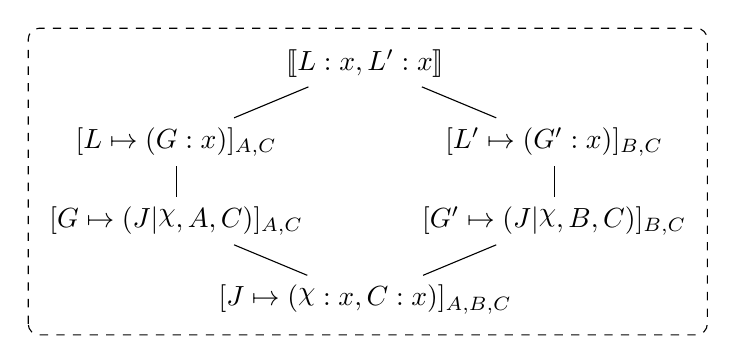
\begin{tikzpicture}[x=2.4cm, y=1cm, framed, background rectangle/.style={draw=black,dashed, rounded corners}] 

  % Specification of nodes (position, etc.)
  \node (a0) at (0,0) { $\adj{\holds{L}{x}{}, \holds{L'}{x}{}}$ };
  \node (b0) at (-1,-1) { $\finalizable{L}{\alloc{G: x}}{A, C}$ };
  \node (b1) at (1,-1) { $\finalizable{L'}{\alloc{G': x}}{B, C}$ };
  \node (g0) at (-1,-2) { $\finalizable{G}{\guar{J}{\rchi, A, C}}{A, C}$ };
  \node (g1) at (1,-2) { $\finalizable{G'}{\guar{J}{\rchi, B, C}}{B, C}$ };
  \node (j) at (0,-3) { $\finalizable{J}{\alloc{\rchi: x, C: x}}{A,B,C}$ };

  \begin{scope}[-]
    \tikzstyle{every node}=[draw=none,below]
    \draw (a0) to (b0);
    \draw (a0) to (b1);
    \draw (b0) to (g0);
    \draw (b1) to (g1);
    \draw (g0) to (j);
    \draw (g1) to (j);
  \end{scope}

\end{tikzpicture}

  \caption{Virtual channel construction}
  \label{fig:virtual-channel-construction}
\end{figure}

We will cover the steps for safely setting up this construction in section \ref{section:open-close-virtual-channel}. 
In the rest of this section we will explain why this construction can be considered to fund the channel $\rchi$.
Similarly to the method for ledger channel construction, we will do this by demonstrating how any one of the participants can offload the channel $\rchi$: converting it to an on-chain channel that holds its own funds.

We will first consider the case where $A$ wishes to offload $\rchi$.
We will assume that $A$ starts by finalizing all their finalizable channels on-chain, followed by a transferring funds held in the ledger channel $L$ to the guarantor channel $G$. 
The final step is for $A$ to claim on $G$'s guarantee for $\rchi$:
\begin{multline}
  \claim{G}{\rchi}{x}\adj{\holds{G}{x}{\guar{J}{\rchi,A,C}}, \holds{L'}{x}{}, \holds{J}{}{\alloc{\rchi: x, C: x}}} =\\
  \adj{\holds{L'}{x}{}, \holds{\rchi}{x}{}, \holds{J}{}{\alloc{C:x}}}
\end{multline}
As $G$ has $\rchi$ as top priority, the operation is successful.

By symmetry, the previous case also covers the case where $B$ wants to offload.
The final case to consider is the one where $C$ wants to offload the channel and reclaim their funds.
This is important to ensure that $A$ and $B$ cannot lock $C$'s funds indefinitely in the channel.
We assume that $C$ has started by registering all their finalizable channels on-chain, followed by transferring funds from $L$ to $G$ and from $L'$ to $G'$.
\begin{multline}
  \claim{G'}{G}{C}\claim{G}{\rchi}{x}\adj{\holds{G}{x}{\guar{J}{\rchi,A,C}}, \holds{G'}{x}{\guar{J}{\rchi, B, C}},\\ \holds{J}{}{\alloc{\rchi: x, C: x}}} =
  \adj{\holds{L'}{x}{}, \holds{\rchi}{x}{}, \holds{C}{x}{}}
\end{multline}
Note that $C$ has to claim on both guarantees, offloading $\rchi$ before being able to reclaim their funds.

As in Turbo, the offload is an action of last resort and virtual channels are designed to be opened and closed entirely off-chain.
We now show how this can be accomplished.

\subsection{Opening and Closing Virtual Channels}\label{section:open-close-virtual-channel}

In this section we present a sequence of system states written in terms of universally finalizable outcomes, where each state differs from the previous state only in one channel.
We claim that this sequence of states can be used to derive a safe procedure for opening a virtual channel, where the value of the system remains unchanged throughout for all participants involved.
We justify this claim in the appendix.

The procedure for opening a virtual channel is as follows:
\begin{enumerate}
  \item Start in the state given in equation (\ref{eq:virtual-channel-start-state}):
  \begin{itemize}
    \item $\adj{\holds{L}{x}{}, \holds{L'}{x}{}}, \; \finalizable{L}{\alloc{A:a, C:b}}{A, C}, \; \finalizable{L'}{\alloc{B: b, C: a}}{B, C}$
  \end{itemize}
  \item $A$ and $B$ bring their channel $\rchi$ to the funding point:
  \begin{itemize}
    \item Create channel $\rchi$: $\finalizable{\rchi}{\alloc{A:a, B:b}}{A,B}$
  \end{itemize}
  \item In any order, $A$, $B$ and $C$ setup the virtual channel construction:
  \begin{itemize}
    \item Create channel $J$: $\finalizable{J}{\alloc{A:a, B:b, C: c}}{A, B, C}$
    \item Create channel $G$: $\finalizable{G}{\guar{J}{\rchi, A, C}}{A, C}$
    \item Create channel $G'$: $\finalizable{G'}{\guar{J}{\rchi, B, C}}{B, C}$
  \end{itemize}
  \item In either order switch the ledger channels over to fund the guarantees:
  \begin{itemize}
    \item Update $L$: $\finalizable{L}{\alloc{G: x}}{A,C}$
    \item Update $L'$: $\finalizable{L'}{\alloc{G': x}}{B,C}$
  \end{itemize}
  \item Switch $J$ over to fund $\rchi$:
  \begin{itemize}
    \item Update channel $J$: $\finalizable{J}{\alloc{\rchi: x, C: x}}{A, B, C}$
  \end{itemize}
\end{enumerate}
We give a visual representation of this procedure in figure \ref{fig:virtual-channel-opening}.

\begin{figure}[ht]
  \centering
  \begin{figure}[h]\centering
  \begin{tikzpicture}[x = 2cm, y=1cm]
    \node (expanded0) at (0, 0) { \begin{tikzpicture}[x=2.4cm, y=1cm, framed, background rectangle/.style={draw=black,dashed, rounded corners}] 
  % Specification of nodes (position, etc.)
  \node (a0) at (0,0) { $\adj{\holds{L}{x}{}, \holds{L'}{x}{}}$ };
  \node (b0) at (-1,-1) { $\finalizable{L}{\alloc{A: a, C: b}}{A, C}$ };
  \node (b1) at (1,-1) { $\finalizable{L'}{\alloc{C:a, B:b}}{B, C}$ };
  \node (g0) at (-1,-2) { $\finalizable{G}{\guar{J}{\rchi, A, C}}{A, C}$ };
  \node (g1) at (1,-2) { $\finalizable{G'}{\guar{J}{\rchi, B, C}}{B, C}$ };
  \node (j) at (0,-3) { $\finalizable{J}{\alloc{A: a, B: b, C: x}}{A, B, C}$ };
  \node (c) at (0,-4) { $\finalizable{\rchi}{\alloc{A:a, B: b}}{A, B}$ };

  \begin{scope}[-]
    \tikzstyle{every node}=[draw=none,below]
    \draw (a0) to (b0);
    \draw (a0) to (b1);
    \draw (g0) to (j);
    \draw (g1) to (j);
  \end{scope}

\end{tikzpicture}
 };
    \node[scale=0.4, rectangle, draw, dashed, rounded corners] (state0) at (3, 1.5) { 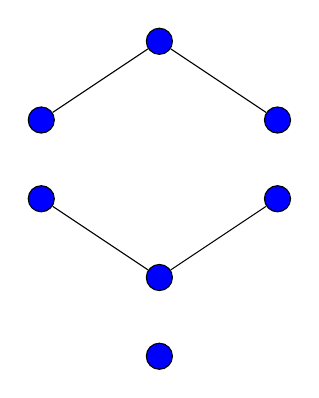
\begin{tikzpicture}[x=1.5cm,y=1cm,every node/.style={draw,solid,shape=circle,fill=blue}]

  % Specification of nodes (position, etc.)
  \node (a0) at (0,0) {};
  \node (b0) at (-1,-1) {};
  \node (b1) at (1,-1) {};
  \node (g0) at (-1,-2) {};
  \node (g1) at (1,-2) {};
  \node (j) at (0,-3) {};
  \node (c) at (0,-4) {};

  \begin{scope}[-]
    \tikzstyle{every node}=[draw,below]
    \draw[solid] (a0) to (b0);
    \draw[solid] (a0) to (b1);
    \draw[solid] (g0) to (j);
    \draw[solid] (g1) to (j);
  \end{scope}

\end{tikzpicture}
 };
    \node[scale=0.4] (state1a) at (4, 1.5) { \input{figures/virtual-channels-mini-1a} };
    \node[scale=0.4] (state1b) at (3, -1) { \input{figures/virtual-channels-mini-1b} };
    \node[scale=0.4] (state2) at (4, -1) { \input{figures/virtual-channels-mini-2} };
    \node[scale=0.4, rectangle, draw, dashed, rounded corners] (state3) at (4, -3.5) { \input{figures/virtual-channels-mini-3} };
    \node (expanded3) at (1, -6) { 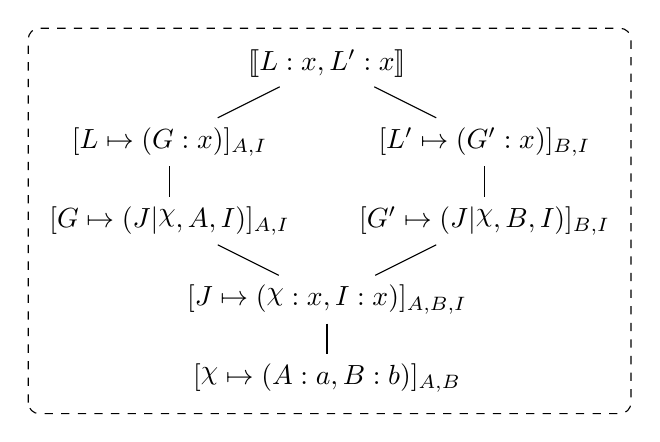
\begin{tikzpicture}[x=2cm, y=1cm, framed, background rectangle/.style={draw=black,dashed, rounded corners}] 

  % Specification of nodes (position, etc.)
  \node (a0) at (0,0) { $\adj{\holds{L}{x}{}, \holds{L'}{x}{}}$ };
  \node (b0) at (-1,-1) { $\finalizable{L}{\alloc{G: x}}{A, I}$ };
  \node (b1) at (1,-1) { $\finalizable{L'}{\alloc{G': x}}{B, I}$ };
  \node (g0) at (-1,-2) { $\finalizable{G}{\guar{J}{\rchi, A, I}}{A, I}$ };
  \node (g1) at (1,-2) { $\finalizable{G'}{\guar{J}{\rchi, B, I}}{B, I}$ };
  \node (j) at (0,-3) { $\finalizable{J}{\alloc{\rchi: x, I: x}}{A,B,I}$ };
  \node (c) at (0,-4) { $\finalizable{\rchi}{\alloc{A: a, B: b}}{A,B}$ };

  \begin{scope}[-]
    \tikzstyle{every node}=[draw=none,below]
    \draw (a0) to (b0);
    \draw (a0) to (b1);
    \draw (b0) to (g0);
    \draw (b1) to (g1);
    \draw (g0) to (j);
    \draw (g1) to (j);
    \draw (j) to (c);
  \end{scope}

\end{tikzpicture}
 };

    \begin{scope}[ultra thick]
      \tikzstyle{every node}=[below]
      \draw[-{Latex[length=3mm,width=4mm]}] (state0) edge (state1a)
                (state0) edge (state1b)
                (state1a) edge (state2)
                (state1b) edge (state2)
                (state2) edge (state3);
    \end{scope}
  \end{tikzpicture}
  \caption{Ledger channels, $x = a + b$}
  \label{fig:modes}
\end{figure} 

  \caption{Opening a virtual channel}
  \label{fig:virtual-channel-opening}
\end{figure}

The same sequence of states, when taken in reverse, can be used to close a virtual channel:
\begin{enumerate}
  \item Participants $A$ and $B$ finalize $\rchi$ by signing a conclusion proof:
  \begin{itemize}
    \item Update $\rchi$: $\finalizable{\rchi}{\alloc{A:a', B:b'}}{A,B}$
  \end{itemize}
  \item $A$ and $B$ sign an update to $J$ to take account of the outcome of $\rchi$. $C$ will accept this update, provided that their allocation of $x$ coins remains the same:
  \begin{itemize}
    \item Update channel $J$: $\finalizable{J}{\alloc{A: a', B:b', C: x}}{A, B, C}$
  \end{itemize}
  \item In either order switch the ledger channels to absorb the outcome of $J$, defunding the guarantor channels in the process:
  \begin{itemize}
    \item Update $L$: $\finalizable{L}{\alloc{A: a', C: b'}}{A,C}$
    \item Update $L'$: $\finalizable{L'}{\alloc{B: b', C: a'}}{B,C}$
  \end{itemize}
  \item The channels $\rchi$, $J$, $G$ and $G'$ are now all defunded, so can be discarded
\end{enumerate}

It is also possible to do top-ups and partial checkouts from a virtual channel.

\section{Acknowledgements}

- Andrew Stewart
- James Prestwich
- Chris Buckland
- Magmo team

\newpage

\section{Appendix}

THIS APPENDIX IS STILL A WIP.

\subsection{Overview of ForceMove}
\subsection{The Consensus Game}

In the presentation of Turbo and Nitro, we will often use the fact that, if you use the
consensus game transition to move between two system states with the same value to a
participant, then all the intermediate states also have the same value to that participant.
This is the key observation that allows us to prove that we can open and close channels
off-chain.

\textbf{Value Preserving Consensus Transitions (VPCTs)}:
If I have two system states, $\Sigma$ and $\Sigma'$, which only differ in the state of
a consensus game chanel, $\rchi$, with participants $P$ and universally enforceable outcomes
$\enf{\Omega_\rchi}_P \in \Sigma$ and $\enf{\Omega'_\rchi}_P \in \Sigma'$, and 
for some participant $p \in P$, $\nu_p(\Sigma) = \nu_p(\Sigma') = x$, then
applying a consensus game transition gives a sequence of system states 
$\Sigma = \Sigma_0, \dots, \Sigma_m = \Sigma'$ where $\nu_p(\Sigma_i) = x$ for all $\Sigma_i$.

Proof (sketch): As $\nu_p(\Sigma) = \nu_p(\Sigma) = x$ and $\Sigma$ and $\Sigma'$ only differ
in $\rchi$, we know that if $p$ can register either outcome $\Omega_\rchi$ or $\Omega'_\rchi$ on-chain, then
they can obtain value $x$. The consensus transition allows the participants to transition
from outcome $\Omega_\rchi$ to $\Omega'_\rchi$ without any participant enabling any other outcome.
Therefore at all points, $p$ is capable of registering one of those outcomes on-chain (though
in general they cannot choose which).
Therefore, at all points, the value of the system to $p$ is $x$.

\subsection{Virtual Channels on Turbo}
\subsection{Payouts to Non-Participants}
\subsection{Possible Extensions}

\subsection{On-chain Operations Code}
\subsubsection{Overlap}
\begin{minipage}{\linewidth} % minipage to avoid page breaks
  \lstinputlisting[language=Python]{code/overlap.py}
\end{minipage}


\end{document}
